\begin{topic}{topological-manifold}{topological manifold}
    A \textbf{topological manifold of dimension $n$} is a \tref{TO:second-countable}{second countable} \tref{TO:hausdorff-space}{Hausdorff} \tref{TO:topological-space}{topological space} in which every point has an open neighborhood that is \tref{TO:homeomorphism}{homeomorphic} to an open subset of $\RR^n$.
\end{topic}

\begin{topic}{atlas}{atlas}
    Let $M$ be a \tref{topological-manifold}{topological manifold}. A \textbf{chart} on $M$ is a pair $(U, \varphi)$ where $U$ is an open subset of $M$ and $\varphi : U \to \tilde{U}$ is a \tref{TO:homeomorphism}{homeomorphism} from $U$ to an open subset $\tilde{U} \subset \RR^n$. An \textbf{atlas} for $M$ is a collection of charts $\{ (U_\alpha, \varphi_\alpha) \}$ such that the $U_\alpha$ cover $M$.
    
    An atlas is \textbf{smooth} if any two charts $(U, \varphi)$ and $(V, \psi)$ are \textit{smoothly compatible}, that is, either $U \cap V = \varnothing$ or the \textit{transition map}
    \[ \psi \circ \varphi^{-1} : \varphi(U \cap V) \to \psi(U \cap V) \]
    is \textit{smooth}: all its continuous partial derivatives exist.
    
    A smooth atlas is \textbf{maximal} if it is not contained in any strictly larger smooth atlas.
\end{topic}

\begin{topic}{smooth-structure}{smooth structure}
    A \textbf{smooth structure} on a \tref{topological-manifold}{topological manifold} $M$ is a \tref{atlas}{maximal smooth atlas} for $M$.
\end{topic}

\begin{topic}{smooth-manifold}{smooth manifold}
    A \textbf{smooth manifold} is \tref{topological-manifold}{topological manifold} $M$ together with a \tref{smooth-structure}{smooth structure} on $M$.
\end{topic}

\begin{topic}{smooth-map}{smooth map}
    A map $f : M \to N$ between \tref{smooth-manifold}{smooth manifolds} is \textbf{smooth} if for all \tref{atlas}{charts} $(U, \varphi)$ of $M$ and $(V, \psi)$ of $N$, the composition
    \[ \psi \circ f \circ \varphi^{-1} : \varphi(f^{-1}(V) \cap U) \to \psi(V) \]
    is \textit{smooth}, i.e. all its continuous partial derivatives exist.
\end{topic}

\begin{topic}{diffeomorphism}{diffeomorphism}
    A \textbf{diffeomorphism} is a \tref{smooth-map}{smooth map} $f : M \to N$ between \tref{smooth-manifold}{smooth manifolds} that has a smooth inverse $f^{-1} : N \to M$.
    
    A \textbf{local diffeomorphism} is a smooth map $f : M \to N$ for which every point $p \in M$ has a neighborhood $U \subset M$ such that $f(U)$ is open in $N$ and $f : U \to f(U)$ is a diffeomorphism.
    
    The manifolds $M$ and $N$ are called \textbf{diffeomorphic} if there exists diffeomorphism between them.
\end{topic}

\begin{topic}{submersion}{submersion}
    A \tref{smooth-map}{smooth map} $f : M \to N$ between \tref{smooth-manifold}{smooth manifolds} is a \textbf{submersion} if the derivative $df_p : T_p M \to T_{f(p)} N$ is surjective for all $p \in M$.
\end{topic}

\begin{topic}{immersion}{immersion}
    A \tref{smooth-map}{smooth map} $f : M \to N$ between \tref{smooth-manifold}{smooth manifolds} is an \textbf{immersion} if the derivative $df_p : T_p M \to T_{f(p)} N$ is injective for all $p \in M$.
\end{topic}

\begin{topic}{embedding}{embedding}
    A \tref{smooth-map}{smooth map} $f : M \to N$ between \tref{smooth-manifold}{smooth manifolds} is an \textbf{embedding} if it is an \tref{immersion}{immersion} and a \tref{TO:homeomorphism}{homeomorphism} onto its image.
\end{topic}

\begin{topic}{tangent-space}{tangent space}
    Let $M$ be a \tref{smooth-manifold}{smooth manifold} and $p$ a point of $M$. A \textbf{derivation at $p$}, or a \textbf{tangent vector at $p$}, is a linear map $v : C^\infty(M) \to \RR$ satisfying
    \[ v(fg) = f(p) v(g) + g(p) v(f) \]
    for all $f, g \in C^\infty(M)$. The \textbf{tangent space} to $M$ at $p$ is the set of all derivations at $p$, denoted $T_p M$. It is a real \tref{LA:vector-space}{vector space} of the same dimension as the dimension of $M$.
\end{topic}

\begin{topic}{tangent-bundle}{tangent bundle}
    Let $M$ be an $n$-dimensional \tref{smooth-manifold}{smooth manifold}. The \textbf{tangent bundle} of $M$, denoted $TM$, is defined as the disjoint union of the \tref{tangent-space}{tangent spaces} at all points of $M$,
    \[ TM = \bigsqcup_{p \in M} T_p M . \]
    It naturally has the structure of a $2n$-dimensional smooth manifold such that the projection map
    \[ \pi : TM \to M, \quad (p, v) \mapsto p \]
    is \tref{smooth-map}{smooth}.
\end{topic}

\begin{topic}{vector-field}{vector field}
    Let $M$ be a \tref{smooth-manifold}{smooth manifold}. A \textbf{vector field} on $M$ is a section of the \tref{tangent-bundle}{tangent bundle} $\pi : TM \to M$, i.e. a map $X : M \to TM$ such that $X(p) \in T_p M$ for all $p \in M$.
\end{topic}

\begin{topic}{cotangent-space}{cotangent space}
    Let $M$ be a \tref{smooth-manifold}{smooth manifold}. The \textbf{cotangent space} to $M$ at a point $p \in M$, denoted $T^*_p M$ is the \tref{LA:dual-vector-space}{dual} of the \tref{tangent-space}{tangent space} $T_p M$,
    \[ T^*_p M = (T_p M)^* . \]
    Elements of $\xi \in T^*_p M$ are called \textbf{tangent covectors} at $p$.
\end{topic}

\begin{topic}{cotangent-bundle}{cotangent bundle}
    Let $M$ be an $n$-dimensional \tref{smooth-manifold}{smooth manifold}. The \textbf{cotangent bundle} of $M$, denoted $T^*M$, is defined as the disjoint union of the \tref{cotangent-space}{cotangent spaces} at all points of $M$,
    \[ T^*M = \bigsqcup_{p \in M} T^*_p M . \]
    It naturally has the structure of a $2n$-dimensional smooth manifold such that the projection map
    \[ \pi : T^*M \to M, \quad (p, \xi) \mapsto p \]
    is \tref{smooth-map}{smooth}.
\end{topic}

\begin{topic}{vector-bundle}{vector bundle}
    Let $M$ be a \tref{smooth-manifold}{smooth manifold}. A \textbf{vector bundle of rank $k$} over $M$ is a smooth manifold $E$ together with a surjective \tref{smooth-map}{smooth map} $\pi : E \to M$ such that
    \begin{itemize}
        \item for each $p \in M$, the \textit{fiber} $E_p = \pi^{-1}(p)$ has the structure of a real \tref{LA:vector-space}{vector space},
        \item for each $p \in M$, there exists a neighborhood $U \subset M$ of $p$ and a \tref{diffeomorphism}{diffeomorphism} $\Phi : \pi^{-1}(U) \to U \times \RR^k$ such that
        \[ \begin{tikzcd} \pi^{-1}(U) \arrow{rr}{\Phi} \arrow[swap]{dr}{\pi} && U \times \RR^k \arrow{dl}{\pi_U} \\ & U & \end{tikzcd} \]
        commutes, and the restriction of $\Phi|_{E_p} : E_p \to \{ p \} \times \RR^k \simeq \RR^k$ is a linear isomorphism.
    \end{itemize}
\end{topic}

\begin{topic}{differential-form}{differential form}
    Let $M$ be a \tref{smooth-manifold}{smooth manifold}. A \textbf{smooth differential $k$-form} is a smooth section of the $k$-th exterior power of the \tref{cotangent-bundle}{cotangent bundle} $\wedge^k T^* M$. The set of all smooth differential $k$-forms is a \tref{LA:vector-space}{vector space} denoted by $\Omega^k(M)$.
\end{topic}

\begin{topic}{exterior-derivative}{exterior derivative}
    Let $M$ be a \tref{smooth-manifold}{smooth manifold}. The \textbf{exterior product} is the unique linear map $d : \Omega^k(M) \to \Omega^{k - 1}(M)$ between \tref{differential-form}{differential forms} satisfying
    \begin{itemize}
        \item for any smooth function $f$ (that is, a $0$-form), $df$ is the \textit{differential} of $f$, that is, $df(X) = X(f)$ for any \tref{vector-field}{vector field} $X$,
        \item $d(df) = 0$ for all smooth functions $f$,
        \item $d(\omega \wedge \eta) = d \omega \wedge \eta + (-1)^k (\omega \wedge d\eta)$ for all $k$-forms $\omega$ and $p$-forms $\eta$.
    \end{itemize}
    It can be shown that $d(d\omega) = 0$ for all $k$-forms $\omega$, which is commonly expressed as $d^2 = 0$.
    
    In local coordinates, if $\omega = \sum_I \omega_I dx^I$ (multi-index notation) then
    \[ d \omega = \sum_I \sum_j \frac{\partial \omega_I}{\partial x^j} dx^j \wedge dx^I . \]
\end{topic}

\begin{example}{exterior-derivative}
    Let $\omega = x^2 \; dy \wedge dz + yz \; dx \wedge dz$ be a $2$-form on $\RR^3$. Then
    \[ \begin{aligned}
        d\omega
            &= 2x \; dx \wedge dy \wedge dz + z \; dy \wedge dx \wedge dz + y \; dz \wedge dx \wedge dz \\
            &= (2x - z) \; dx \wedge dy \wedge dz .
    \end{aligned} \]
\end{example}

\begin{topic}{interior-product}{interior product}
    Let $M$ be a \tref{smooth-manifold}{smooth manifold}. The \textbf{interior product} is the \textit{contraction} of a \tref{differential-form}{differential form} with a \tref{vector-field}{vector field}. That is, if $X$ is a vector field on $M$, then
    \[ \iota_X : \Omega^k(M) \to \Omega^{k - 1} \]
    is the map defined by
    \[ (\iota_X \omega)(Y_1, \ldots, Y_{k - 1}) = \omega(X, Y_1, \ldots, Y_{k - 1}) \]
    for any vector fields $Y_1, \ldots, Y_{k - 1}$.
\end{topic}

\begin{topic}{lie-derivative}{Lie derivative}
    Let $M$ be a \tref{smooth-manifold}{smooth manifold}. The \textbf{Lie derivative} of a \tref{tensor-field}{tensor field} $T$ with respect to a \tref{vector-field}{vector field} $X$ is the tensor field $\mathcal{L}_X T$ (of the same type as $T$), given by
    \[ (\mathcal{L}_X T)_p = \frac{d}{dt}\Big|_{t = 0} \left( \left(\varphi^t_X\right)^* T \right)_p \]
    for all points $p \in M$. Here $\varphi^t_X$ denotes the flow of $X$.
\end{topic}

\begin{example}{lie-derivative}
    When $f$ is a smooth function, we have
    \[ \begin{aligned}
        (\mathcal{L}_X f)(p)
            &= \frac{d}{dt}\Big|_{t = 0} \left(\left(\varphi^t_X\right)^* f \right)(p) \\
            &= \frac{d}{dt}\Big|_{t = 0} f \left(\varphi^t_X(p)\right) \\
            &= df_p \left( \frac{d}{dt}\Big|_{t = 0} \varphi^t_X(p) \right) \\
            &= df_p(X_p) \\
            &= X(f)(p) .
    \end{aligned} \]
    
\end{example}

\begin{topic}{lie-bracket-vector-fields}{Lie bracket of vector fields}
    Let $M$ be a \tref{smooth-manifold}{smooth manifold}. The \textbf{Lie bracket} of two \tref{vector-field}{vector fields} $X, Y$ is defined as the vector field $[X, Y]$ given by
    \[ [X, Y](f) = X(Y(f)) - Y(X(f)) \]
    for all smooth functions $f$ on $M$.
\end{topic}

\begin{topic}{cartan-formula}{Cartan formula}
    The \textbf{Cartan formula} relates the \tref{interior-product}{interior product}, \tref{exterior-derivative}{exterior derivative} and \tref{lie-derivative}{Lie derivative} via
    \[ \mathcal{L}_X \omega = d(\iota_X \omega) + \iota_X d \omega . \]
\end{topic}

\begin{topic}{closed-form}{closed form}
    Let $M$ be a \tref{smooth-manifold}{smooth manifold}. A \tref{differential-form}{differential form} $\omega$ is \textbf{closed} if its \tref{exterior-derivative}{exterior derivative} is zero, that is, if $dw = 0$.
\end{topic}

\begin{topic}{exact-form}{exact form}
    Let $M$ be a \tref{smooth-manifold}{smooth manifold}. A \tref{differential-form}{differential form} $\omega$ is \textbf{exact} if it is the \tref{exterior-derivative}{exterior derivative} of another differential form $\eta$, that is, if $\omega = d \eta$.
\end{topic}

\begin{topic}{tensor-field}{tensor field}
    Let $M$ be a \tref{smooth-manifold}{smooth manifold}. A \textbf{tensor bundle} on $M$ is any \tref{vector-bundle}{vector bundle} of the form
    \[ \underbrace{TM \otimes \cdots TM}_{p \text{ times}} \otimes \underbrace{T^*M \otimes \cdots T^*M}_{q \text{ times}} . \]
    A \textbf{tensor field} of \textit{type} $(p, q)$ is a section of this bundle.
\end{topic}

\begin{topic}{parallelizable-manifold}{parallelizable manifold}
    A \tref{smooth-manifold}{smooth manifold} $M$ is \textbf{parallelizable} if its \tref{tangent-bundle}{tangent bundle} $TM$ is trivial, that is, $TM$ is \tref{diffeomorphism}{diffeomorphic} to $M \times \RR^n$.
\end{topic}

\begin{topic}{inverse-function-theorem}{inverse function theorem}
    The \textbf{inverse function theorem} states that if $f : M \to N$ is a \tref{smooth-map}{smooth map} between \tref{smooth-manifold}{smooth manifolds}, whose derivative $df_p : T_p M \to T_{f(p)} N$ at some point $p \in M$ is an isomorphism, then $f$ is a \tref{diffeomorphism}{local diffeomorphism} at $p$.
\end{topic}

\begin{topic}{partition-of-unity}{partition of unity}
    Let $M$ be a \tref{smooth-manifold}{smooth manifold}. A \textbf{partition of unity} on $M$ is a set of smooth functions $\{ f_\alpha : M \to [0, 1] \}$ so that each point $p \in M$ has a neighborhood where only finitely many $f_\alpha$ are nonzero and $\sum_\alpha f_\alpha(p) = 1$.
    
    It is a theorem that for any open cover $\{ U_\alpha \}$ of $M$, there exists a partition of unity $\{ f_\alpha \}$ such that the support of $f_\alpha$ is contained in $U_\alpha$.
\end{topic}

\begin{topic}{whitney-embedding-theorem}{Whitney embedding theorem}
    The \textbf{Whiteney embedding theorem} states that any \tref{smooth-manifold}{smooth $n$-dimensional manifold} can be \tref{embedding}{embedded} in $\RR^{2n}$, for all $n > 0$.
\end{topic}

\begin{example}{whitney-embedding-theorem}
    The dimension $2n$ is a sharp lower bound: projective space $\RR P^n$ cannot be embedded in $\RR^{2n - 1}$ whenever $n$ is a power of $2$.
\end{example}

\begin{topic}{riemannian-manifold}{Riemannian manifold}
    Let $M$ be a \tref{smooth-manifold}{smooth manifold}. A \textbf{Riemannian metric} on $M$ is a smooth symmetric \tref{tensor-field}{$(0, 2)$-tensor field} $g$ that is positive definite at each point $p \in M$. The pair $(M, g)$ is called a \textbf{Riemannian manifold}.
\end{topic}

\begin{topic}{almost-complex-structure}{almost complex manifold}
    Let $M$ be a \tref{smooth-manifold}{smooth manifold}. An \textbf{almost complex structure} on $M$ is a smooth \tref{tensor-field}{tensor field} $J \in \Gamma(TM \otimes T*M)$ satisfying $J^2 = -1$ when viewed as a bundle isomorphism $J : TM \to TM$. The pair $(M, J)$ is called an \textbf{almost complex manifold}.
\end{topic}

\begin{topic}{kahler-manifold}{Kähler manifold}
    A \textbf{Kähler manifold} is a \tref{smooth-manifold}{smooth manifold} $M$ with three compatible structures: a complex structure $J$, a \tref{riemannian-manifold}{Riemannian structure} $g$, and a \tref{symplectic-manifold}{symplectic structure} $\omega$. Compatibility means that
    \[ g(X, Y) = \omega(X, JY) \]
    for all \tref{vector-field}{vector fields} $X, Y$ on $M$.
    
    Note that two-out-of-three structures determines the other structure.
\end{topic}

\begin{topic}{connection}{connection}
    Let $\pi : E \to M$ be a \tref{vector-bundle}{vector bundle} over a \tref{smooth-manifold}{smooth manifold} $M$. A \textbf{connetion} on $E$ is a linear differential operator
    \[ \nabla : \Gamma(E) \to \Gamma(T^*M \otimes E) \]
    satisfying the \textit{Leibniz rule}
    \[ \nabla(fs) = df \otimes s + f \nabla s \]
    for all smooth functions $f$ and sections $s \in \Gamma(E)$.
\end{topic}

\begin{topic}{curvature-connection}{curvature of a connection}
    Let $\nabla$ be a \tref{connection}{connection} on a \tref{vector-bundle}{vector bundle} $\pi : E \to M$. The map $\nabla^2 : \Omega^0(M; E) \to \Omega^2(M; E)$ is $C^\infty(M)$-linear and hence induced by a section $F_\nabla \in \Omega^2(M; \text{End}(E))$, called the \textbf{curvature} of $\nabla$.
\end{topic}

\begin{topic}{flat-connection}{flat connection}
    A \tref{connection}{connection} $\nabla$ on a \tref{vector-bundle}{vector bundle} $\pi : E \to M$ is \textbf{flat} if its \tref{curvature-connection}{curvature} is zero.
\end{topic}

\begin{topic}{curvature-form}{curvature form}
    Let $\nabla$ be a \tref{connection}{connection} on a \tref{vector-bundle}{vector bundle} $\pi : E \to M$. The \textbf{curvature form} of $E$ is the $2$-form $k(E) = \frac{1}{2 \pi i} \text{tr } F_\nabla \in \Omega^2(M)$, where $F_\nabla \in \Omega^2(M; \text{End}(M))$ is the \tref{curvature-connection}{curvature} of $\nabla$. It is a \tref{closed-form}{closed form} and the corresponding cohomology class $\kappa(E) = [k(E)] \in H_\text{dR}^2(M)$ is called the \textbf{curvature class} of $E$.
\end{topic}

\begin{topic}{torsion-connection}{torsion of connection}
    Let $M$ be a \tref{smooth-manifold}{smooth manifold} with a \tref{connection}{connection} $\nabla$ on the \tref{tangent-bundle}{tangent bundle} $TM$ of $M$. The \textbf{torsion} of $\nabla$ is the tensor $T \in \Gamma(TM \otimes \wedge^2 T^* M)$ given by
    \[ T_\nabla(X, Y) = \nabla_X Y  - \nabla_Y X - [X, Y] , \]
    where $[X, Y]$ denotes the \tref{lie-bracket-vector-fields}{Lie bracket of vector fields}.
    
    The connection $\nabla$ is called \textit{torsion-free} if $T_\nabla = 0$.
\end{topic}

\begin{topic}{levi-civita-connection}{Levi-Civita connection}
    Let $(M, g)$ be a \tref{riemannian-manifold}{Riemannian manifold}. The \textbf{Levi-Civita connection} is the unique \tref{connection}{connection} on the \tref{tangent-bundle}{tangent bundle} that preserves the metric $g$, i.e. $\nabla g = 0$, and is \tref{torsion-connection}{torsion-free}.
\end{topic}

\begin{topic}{christoffel-symbols}{Christoffel symbols}
    Let $(M, g)$ be a \tref{riemannian-manifold}{Riemannian manifold}. The \textbf{Christoffel symbols} ${\Gamma^k}_{ij}$ are the connection coefficients (in a given coordinate basis) of the \tref{levi-civita-connection}{Levi-Civita connection}. That is, they are the unique coefficients such that
    \[ \nabla_{\partial_i} \partial_j = {\Gamma^k}_{ij} \partial_k , \]
    where the $\partial_i$ denote a local coordinate basis, and $\nabla$ the Levi-Civita connection.
    
    The Christoffel symbols can be computed from the metric $g$ via
    \[ {\Gamma^k}_{ij} = \frac{1}{2} g^{k \ell} \left(\frac{\partial g_{\ell i}}{\partial x^j} + \frac{\partial g_{\ell j}}{\partial x^i} - \frac{\partial g_{ij}}{\partial x^\ell} \right) . \]
\end{topic}

\begin{topic}{parallel-transport}{parallel transport}
    Let $M$ be a \tref{smooth-manifold}{smooth manifold}, and $E \to M$ a \tref{vector-bundle}{vector bundle} on $M$ with \tref{connection}{connection} $\nabla$. A section $s : M \to E$ is called \textbf{parallel} if $\nabla s = 0$.
    
    The problem of parallel transport asks, given a point $p \in M$ and vector $v \in E_p$, if there exists (locally) a section $s : U \to E$ such that $\nabla s = 0$ and $s(p) = v$, for some neighborhood $U \subset M$ of $p$. If it exists, this section is called the \textbf{parallel transport} of $v$. It is a theorem that this can be done for all $p$ and $v$ if and only if the \tref{curvature-connection}{curvature} $F_\nabla$ vanishes.
\end{topic}

\begin{example}{parallel-transport}
    In particular, given a path $\gamma : [0, 1] \to M$, the connection $\gamma^* \nabla$ on $\gamma^* E$ must have zero curvature since $F_{\gamma^* \nabla}$ is a $2$-form. Therefore, for any starting vector $v \in E_{\gamma(0)}$ there is a unique section $s \in \Gamma(\gamma^* E)$ such that $s(0) = v$ and $(\gamma^* \nabla) s = 0$.
\end{example}

\begin{topic}{affine-connection}{affine connection}
    Let $M$ be a \tref{smooth-manifold}{smooth manifold}. An \textbf{affine connection} on $M$ is a \tref{connection}{connection} on the \tref{tangent-bundle}{tangent bundle} $TM$ of $M$.
\end{topic}

\begin{topic}{distribution}{distribution}
    Let $M$ be a \tref{smooth-manifold}{smooth manifold}. A \textbf{distribution} on $M$ is a vector subbundle $\mathcal{D} \subset TM$.
\end{topic}

\begin{example}{distribution}
    If $M$ has a nowhere vanishing vector field $X$, the subbundle $\mathcal{D} \subset TM$ generated (fiberwise) by $X$ is a rank one distribution.
\end{example}

\begin{example}{distribution}
    Given a \tref{submersion}{submersion} $f : N \to M$, the subbundle $\ker(f_*) \subset TN$ is a distribution on $N$ of rank $\dim N - \dim M$.
\end{example}

\begin{topic}{integral-submanifold}{integral submanifold}
    Let $M$ be a \tref{smooth-manifold}{smooth manifold}. Given a rank $k$ \tref{distribution}{distribution} $\mathcal{D} \subset TM$ and a point $p \in M$, an \textbf{integral submanifold} of $\mathcal{D}$ through $p$ is an \tref{immersion}{immersion} of a $k$-dimensional manifold $i : N \to M$ such that $p \in i(N)$ and for all $q \in N$ one has $i_*(T_q N) = \mathcal{D}_{i(q)}$.
\end{topic}

\begin{topic}{integral-distribution}{integral distribution}
    A \tref{distribution}{distribution} $\mathcal{D} \subset TM$ on a \tref{smooth-manifold}{smooth manifold} $M$ is \textbf{integrable} if for every $p \in M$ there exists an \tref{integral-submanifold}{integral submanifold} of $\mathcal{D}$ through $p$.
\end{topic}

\begin{topic}{involutive-distribution}{involutive distribution}
    A \tref{distribution}{distribution} $\mathcal{D} \subset TM$ on a \tref{smooth-manifold}{smooth manifold} $M$ is \textbf{involutive} if for all $X, Y \in \Gamma(\mathcal{D})$, the \tref{lie-bracket-vector-fields}{Lie bracket} $[X, Y] \in \Gamma(\mathcal{D})$.
\end{topic}

\begin{example}{involutive-distribution}
    Every \tref{integral-distribution}{integral distribution} is involutive. Indeed, at any point $p \in M$ there exists an \tref{integral-submanifold}{integral submanifold} $i : N \to M$, so that $X, Y \in \Gamma(\mathcal{D})$ can be viewed as vector fields on $N$. Hence, $[X, Y]$ is also a vector field on $N$.
    
    Conversely, it is a theorem by Frobenius that every involutive distribution is integrable.
\end{example}

\begin{topic}{vertical-distribution}{vertical distribution}
    Let $M$ be a \tref{smooth-manifold}{smooth manifold} and $p : E \to M$ a \tref{vector-bundle}{vector bundle} on $M$. Then the \textbf{vertical distribution} on $E$ is the \tref{distribution}{distribution} $\mathcal{V} = \ker(p_*) \subset TE$, whose rank is the rank of $E$.
\end{topic}

\begin{topic}{horizontal-distribution}{horizontal distribution}
    Let $M$ be a \tref{smooth-manifold}{smooth manifold} and $p : E \to M$ a \tref{vector-bundle}{vector bundle} on $M$ with a \tref{connection}{connection} $\nabla$. Then the \textbf{horizontal distribution} on $E$ is the \tref{distribution}{distribution} $\mathcal{H} \subset TE$ given by
    \[ \mathcal{H}_x = \left\{ \frac{d}{dt}\Big|_{t = 0} s(t) : s : [-1, 1] \to E \text{ with } s(0) = x \text{ is a parallel section over } \gamma = p \circ s \right\} \]
    for all points $x \in E$.
    
    That is, a section $s : M \to E$ is \tref{parallel-transport}{parallel} if and only if it is an \tref{integral-submanifold}{integral submanifold} of $\mathcal{H}$.
\end{topic}

\begin{topic}{geodesic}{geodesic}
    Let $M$ be a \tref{smooth-manifold}{smooth manifold} and $\nabla$ a \tref{connection}{connection} on $TM$. A \textbf{geodesic} is a curve $\gamma : I \to M$ such that $(\gamma^* \nabla) \gamma' = 0$. That is, a curve which \tref{parallel-transport}{parallel transports} its own tangent direction.
\end{topic}

\begin{example}{geodesic}
    Suppose that $\nabla$ is the \tref{levi-civita-connection}{Levi-Civita connection} on $M$. Then in terms of local coordinates, the differential equation for a geodesic $\gamma : I \to M$ is given by
    \[ \frac{d^2 x^k}{d t^2} + {\Gamma^k}_{ij} \frac{dx^i}{dt} \frac{dx^j}{dt} = 0 , \]
    where ${\Gamma^k}_{ij}$ denote the \tref{christoffel-symbols}{Christoffel symbols}.
\end{example}

% ---

\begin{topic}{de-rham-isomorphism}{de Rham isomorphism}
    The \textbf{de Rham isomorphism} is the isomorphism given by
    \[ H_{\textup{dR}}^k(X) \xrightarrow{\sim} H^k(X; \RR) : [ \omega ] \mapsto \int_{(-)} \omega . \]
    The exterior product endows the direct sum of these groups with a ring structure. A further result of the theorem is that the two cohomology rings are isomorphic (as \tref{CA:graded-ring}{graded rings}), where the analogous product on \tref{AT:singular-homology}{singular cohomology} is the \tref{AT:cup-product}{cup product}.
\end{topic}

\begin{topic}{poincare-duality}{Poincaré duality}
    Let $X$ be a compact oriented $n$-dimensional manifold. \textbf{Poincaré duality} states that there is a canonical isomorphism
    \[ H^k(X; \ZZ) \xrightarrow{\sim} H_{n - k}(X; \ZZ) \]
    which sends $\omega$ to the cap product $[X] \frown \omega$, where $[X] \in H_n(X; \ZZ)$ denotes the fundamental class of $X$. That is, $\omega$ is sent to
    \[ (\eta \mapsto (\omega \smile \eta)([X])) \in \Hom(H^{n - k}(X; \ZZ), \ZZ) = H_{n - k}(X; \ZZ) . \]
\end{topic}

\begin{topic}{fundamental-class}{fundamental class}
    The \textbf{fundamental class} of a closed orientable $n$-dimensional manifold $M$ is a homology class $[M] \in H_n(M; \ZZ)$ which is a generator of the homology group corresponding to the orientation of $M$.
\end{topic}

\begin{topic}{exponential-map}{exponential map}
    Let $M$ be a \tref{smooth-manifold}{smooth manifold} with a \tref{connection}{connection} $\nabla$ on the \tref{tangent-bundle}{tangent bundle} $TM$, and $p \in M$ a point. Any \tref{tangent-space}{tangent vector} $v \in T_p M$ induces a \tref{geodesic}{geodesic} $\gamma : [0, 1] \to M$ starting at $\gamma(0) = p$ with velocity $\gamma'(0) = v$. The \textbf{exponential map} at $p$ is the map
    \[ \exp : T_p M \to M, \quad v \mapsto \gamma(1) . \]
\end{topic}

\begin{example}{exponential-map}
    When $G$ is a \tref{lie-group}{Lie group}, the exponential map is the map
    \[ \exp : \mathfrak{g} \to G \]
    from Lie algebra $\mathfrak{g} = T_e G$ of $G$ to $G$, given by $\exp(v) = \gamma(1)$ where $\gamma : \RR \to G$ is the unique one-parameter subgroup of $G$ with $\gamma'(0) = v$.
    
    In particular, when $G = \text{GL}_n(\RR)$ is the general linear group, we have $\mathfrak{g} = \text{Mat}_{n \times n}(\RR)$ and
    \[ \exp : \mathfrak{g} \to G, \quad A \mapsto \exp(A) = \sum_{k = 0}^{\infty} \frac{A^k}{k!} \]
    is the usual \tref{LA:matrix-exponential}{exponential map}.
\end{example}

\begin{topic}{closed-manifold}{closed manifold}
    A \textbf{closed manifold} is a \tref{smooth-manifold}{manifold} without boundary that is \tref{TO:compact-space}{compact}.
\end{topic}

\begin{topic}{bordism}{bordism}
    Given two $(n - 1)$-dimensional \tref{closed-manifold}{closed} \tref{smooth-manifold}{smooth manifolds} $M$ and $M'$, a \textbf{bordism} from $M$ to $M'$ is an $n$-dimensional compact manifold $W$ with boundary together with inclusions
    \[ M \xrightarrow{i} W \xleftarrow{i'} M' \]
    such that $\partial W = i(M) \sqcup i(M')$.
\end{topic}

\begin{example}{bordism}
    The following are visual examples of $2$-dimensional bordisms.
    \[  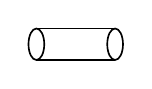
\begin{tikzpicture}[semithick, scale=0.5, baseline=-0.5ex] \begin{scope} \draw (-1,0) ellipse (0.2cm and 0.4cm); \draw (-1,0.4) -- (1,0.4); \draw (-1,-0.4) -- (1,-0.4); \draw (1,0) ellipse (0.2cm and 0.4cm); \end{scope} \end{tikzpicture}
        \quad
        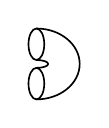
\begin{tikzpicture}[semithick, scale=0.5, baseline=-0.5ex] \begin{scope} \draw (0,0.5) ellipse (0.2cm and 0.4cm); \draw (0,-0.5) ellipse (0.2cm and 0.4cm); \draw (0,0.9) arc (90:-90:1.1cm and 0.9cm); \draw (0,0.1) arc (90:-90:0.3cm and 0.1cm); \end{scope} \end{tikzpicture}
        \quad
        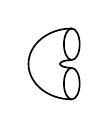
\begin{tikzpicture}[semithick, scale=0.5, baseline=-0.5ex] \begin{scope} \draw (0,0.5) ellipse (0.2cm and 0.4cm);\draw (0,-0.5) ellipse (0.2cm and 0.4cm); \draw (0,0.9) arc (90:270:1.1cm and 0.9cm); \draw (0,0.1) arc (90:270:0.3cm and 0.1cm); \end{scope} \end{tikzpicture}
        \quad
        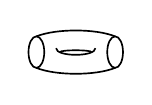
\begin{tikzpicture}[semithick, scale=0.5, baseline=-0.5ex] \begin{scope} \draw (-1,0) ellipse (0.2cm and 0.4cm); \draw (-1,0.4) .. controls (-0.5,0.6) and (0.5,0.6) .. (1,0.4); \draw (-1,-0.4) .. controls (-0.5,-0.6) and (0.5,-0.6) .. (1,-0.4); \draw (-0.5,0.1) .. controls (-0.5,-0.125) and (0.5,-0.125) .. (0.5,0.1); \draw (-0.4,0.0) .. controls (-0.4,0.0625) and (0.4,0.0625) .. (0.4,0.0); \draw (1,0) ellipse (0.2cm and 0.4cm); \end{scope} \end{tikzpicture}
        \quad
        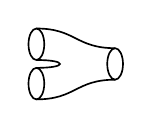
\begin{tikzpicture}[semithick, scale=0.5, baseline=-0.5ex] \begin{scope} \draw (-1,0.5) ellipse (0.2cm and 0.4cm); \draw (-1,-0.5) ellipse (0.2cm and 0.4cm); \draw (1,0) ellipse (0.2cm and 0.4cm); \draw (-1,0.9) .. controls (0,0.9) and (0,0.4) .. (1,0.4); \draw (-1,-0.9) .. controls (0,-0.9) and (0,-0.4) .. (1,-0.4); \draw (-1,0.1) .. controls (-0.2,0.1) and (-0.2,-0.1) .. (-1,-0.1); \end{scope} \end{tikzpicture}
        \quad
        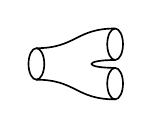
\begin{tikzpicture}[semithick, scale=0.5, baseline=-0.5ex] \begin{scope} \draw (-1,0) ellipse (0.2cm and 0.4cm); \draw (1,0.5) ellipse (0.2cm and 0.4cm); \draw (1,-0.5) ellipse (0.2cm and 0.4cm); \draw (-1,0.4) .. controls (0,0.4) and (0,0.9) .. (1,0.9); \draw (-1,-0.4) .. controls (0,-0.4) and (0,-0.9) .. (1,-0.9); \draw (1,0.1) .. controls (0.2,0.1) and (0.2,-0.1) .. (1,-0.1); \end{scope} \end{tikzpicture}
        \quad
        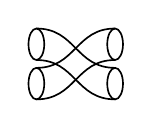
\begin{tikzpicture}[semithick, scale=0.5, baseline=-0.5ex] \begin{scope} \draw (-1,0.5) ellipse (0.2cm and 0.4cm); \draw (-1,-0.5) ellipse (0.2cm and 0.4cm); \draw (1,0.5) ellipse (0.2cm and 0.4cm); \draw (1,-0.5) ellipse (0.2cm and 0.4cm); \draw (-1,0.9) .. controls (0,0.9) and (0,-0.1) .. (1,-0.1); \draw (-1,0.1) .. controls (0,0.1) and (0,-0.9) .. (1,-0.9); \draw (-1,-0.9) .. controls (0,-0.9) and (0,0.1) .. (1,0.1); \draw (-1,-0.1) .. controls (0,-0.1) and (0,0.9) .. (1,0.9); \end{scope} \end{tikzpicture} \]
\end{example}

\begin{example}{bordism}
    Given bordisms $W : M \to M'$ and $W' : M' \to M''$, it can be shown that $W \sqcup_{M'} W'$ admits a smooth structure such that the inclusions $W \to W \sqcup_{M'} W'$ and $W' \to W \sqcup_{M'} W'$ are diffeomorphisms onto their images, which is unique up to (non-unique) diffeomorphism. Hence $W$ and $W'$ can be `composed' to produce a bordism $W' \circ W : M \to M''$, which is well-defined up to isomorphism.
    
    Using this composition rule, one can define the \textit{category of $n$-bordisms} $\textbf{Bord}_n$, where the objects are $(n - 1)$-dimensional closed manifolds and where the morphisms are bordsims are taken up to isomorphism. In particular, the identity morphism of an object $M$ is the cylinder $\id_M = M \times [0, 1]$.
\end{example}

\begin{topic}{lie-algebroid}{Lie algebroid}
    Let $M$ be a \tref{smooth-manifold}{smooth manifold}. A \textbf{Lie algebroid} over $M$ is a \tref{vector-bundle}{vector bundle} $L$ on $M$ together with a \tref{AA:lie-algebra}{Lie bracket} $[\cdot, \cdot]$ on its global sections $\Gamma(L)$ and a map of vector bundles $a : L \to TM$, called the \textit{anchor map}, to the \tref{tangent-bundle}{tangent bundle} of $M$, satisfying
    \begin{itemize}
        \item (\textit{Lie algebra homomorphism}) $a([X, Y]) = [a(X), a(Y)]$ for all $X, Y \in \Gamma(L)$,
        \item (\textit{Leibniz rule}) $[X, fY] = f[X, Y] + (a(X)  f) Y$ for all $X, Y \in \Gamma(L)$ and $f \in C^\infty(M)$.
    \end{itemize}
\end{topic}

\begin{example}{lie-algebroid}
    The tangent bundle $TM$ itself is a Lie algebroid, with the anchor map the identity $\id : TM \to TM$, and Lie bracket the \tref{lie-bracket-vector-fields}{Lie bracket for vector fields}.
\end{example}

\begin{example}{lie-algebroid}
    Given a vector bundle $E \to M$, its \textit{general linear algebroid} is the vector bundle $\mathfrak{gl}(E) \to M$ whose sections are derivations $D : \Gamma(E) \to \Gamma(E)$ of $E$ admitting a vector field $X_D \in TM$ such that $D(f s) = f D(s) + (X_D f) s$ for all $s \in \Gamma(E)$ and $f \in C^\infty(M)$. The Lie bracket is the commutator of differential operators, and the anchor map is the map $D \mapsto X_D$.
\end{example}

\begin{topic}{foliation}{foliation}
    Let $M$ be an $n$-dimensional \tref{smooth-manifold}{smooth manifold}. A $p$-dimensional \textbf{foliation} of $M$ is a decomposition of $M$ into a union of disjoint connected submanifolds
    \[ M = \bigsqcup_{\alpha \in A} L_\alpha \]
    such that each point $x \in M$ has a neighborhood $U$ with local coordinates $x^1, \ldots, x^n$ such that $x^{p + 1}, \ldots, x^n$ are constant on $U \cap L_\alpha$ for all $\alpha \in A$. The submanifolds $L_\alpha$ are called the \textbf{leaves} of the foliation, and the foliation is denoted as $\mathcal{F} = \{ L_\alpha \}_{\alpha \in A}$.
\end{topic}

\begin{topic}{higgs-bundle}{Higgs bundle}
    Let $M$ be a complex manifold. A \textbf{Higgs bundle} on $M$ is a holomorphic vector bundle $E$ on $M$ together with a section $\phi \in \Omega^1(M; \text{End}(E))$, called the \textbf{Higgs field}, satisfying $\phi \wedge \phi = 0$.
\end{topic}

\begin{topic}{frame-bundle}{(tangent) frame bundle}
    The \textbf{frame bundle} of a \tref{vector-bundle}{vector bundle} $E \to M$ of rank $k$ is the vector bundle $F(E) \to M$ whose fibers $F_x$ at a point $x \in M$ is the vector space of ordered bases $\{ e_1, \ldots, e_k \}$ of $E_x$.
    
    There is a natural fiber-wise action of $\text{GL}_k(\RR)$ on $F(E)$ given by change of basis: $\{ e_1, \ldots, e_k \} \cdot g = \{ f_1, \ldots, f_k \}$ where $f_i = \sum_j e_j g_{ji}$. This makes $F(E)$ into a \tref{TO:principal-bundle}{$\text{GL}_k(\RR)$-principal bundle}.
    
    When $E = TM$, the \tref{tangent-bundle}{tangent bundle}, the frame bundle $F(TM)$ is called the \textbf{tangent frame bundle}.
\end{topic}

\begin{topic}{spin-structure}{spin structure}
    Let $(M, g)$ be an $n$-dimensional orientable \tref{riemannian-manifold}{Riemannian manifold}. A \textbf{spin structure} on $M$ is a \tref{TO:principal-bundle}{principal $\text{Spin}(n)$-bundle} $P \to M$ together with a bundle morphism $f : P \to F_{\text{SO}(n)}(M)$ to the oriented orthonormal \tref{frame-bundle}{tangent frame bundle}, equivariant with respect to the double cover $\text{Spin}(n) \to \text{SO}(n)$.
    % Can be generalized to any vector bundle
\end{topic}

\begin{topic}{first-stiefel-whitney-class}{first Stiefel--Whitney class}
    Let $M$ be a \tref{smooth-manifold}{smooth manifold}. There exists a bijection between real line bundles $E \to M$ which can be trivialized over an open cover $\mathcal{U}$ and $\check{H}^1(M, C^\infty(M, \RR^*); \mathcal{U})$, in terms of the transition functions. The group isomorphism
    \[ C^\infty(M, \RR) \times \ZZ_2 \to C^\infty(M, \RR^*), \quad (f, \varepsilon) \mapsto \varepsilon e^f \]
    yields an isomorphism of \tref{AG:cech-cohomology}{Čech cohomology} groups
    \[ \check{H}^k(M; C^\infty(M, \RR); \mathcal{U}) \times \check{H}^k(M; \ZZ_2; \mathcal{U}) \to \check{H}^k(M; C^\infty(M, \RR^*); \mathcal{U}) , \]
    which for $k > 0$ specializes to an isomorphism
    \[ \check{H}^k(M; \ZZ_2; \mathcal{U}) \xrightarrow{\sim} \check{H}^k(M; C^\infty(M, \RR^*); \mathcal{U}) . \]
    The \textbf{first Stiefel--Whitney class} of a real line bundle $E \to M$ is its corresponding class $w_1(E) \in \check{H}^1(M; \ZZ_2; \mathcal{U})$.
    
    The \textbf{first Stiefel--Whitney class} of a rank $k$ real vector bundle $E \to M$ is the first Stiefel--Whitney class of $\wedge^k E$.
\end{topic}

\begin{topic}{first-chern-class}{first Chern class}
    Let $M$ be a \tref{smooth-manifold}{smooth manifold}. There exists a bijection between complex line bundles $E \to M$ which can be trivialized over an open cover $\mathcal{U}$ and $\check{H}^1(M, C^\infty(M, \CC^*); \mathcal{U})$, in terms of the transition functions. The exponential sequence
    \[ 0 \to \ZZ \xrightarrow{2 \pi i} C^\infty(M, \CC) \xrightarrow{\exp} C^\infty(M, \CC^*) \to 0 \]
    yields a long exact sequence of \tref{AG:cech-cohomology}{Čech cohomology} groups
    \[ \cdots \to \check{H}^k(M; \ZZ; \mathcal{U}) \to \check{H}^k(M; C^\infty(M, \CC); \mathcal{U}) \to \check{H}^k(M; C^\infty(M, \CC^*); \mathcal{U}) \to \check{H}^{k + 1}(M; \ZZ; \mathcal{U}) \to \cdots \]
    which in particular gives an isomorphism
    \[ \check{H}^1(M; C^\infty(M, \CC^*); \mathcal{U}) \xrightarrow{\sim} \check{H}^2(M; C^\infty(M, \ZZ; \mathcal{U}) . \]
    The \textbf{first Chern class} of a complex line bundle $E \to M$ is its corresponding class $c_1(E) \in \check{H}^2(M; \ZZ; \mathcal{U})$.
    
    The \textbf{first Chern class} of a rank $k$ complex vector bundle $E \to M$ is the first Chern class of $\wedge^k E$.
\end{topic}

\begin{topic}{determinant-bundle}{determinant bundle}
    The \textbf{determinant bundle} of a \tref{vector-bundle}{vector bundle} $E \to M$ of rank $k$ is the exterior power $\det(E) = \wedge^k E$.
\end{topic}

\begin{topic}{riemann-surface}{Riemann surface}
    A \textbf{Riemann surface} is a \tref{TO:connected-space}{connected} complex manifold of complex dimension one.
\end{topic}

\begin{topic}{volume-form}{volume form}
    Let $M$ be an $n$-dimensional \tref{smooth-manifold}{smooth manifold}. A \textbf{volume form} on $M$ is an \tref{differential-form}{$n$-form} $\omega \in \Omega^n(M)$.
\end{topic}

\begin{example}{volume-form}
    When $M$ is a \tref{riemannian-manifold}{Riemannian manifold} with metric $g$, there is a natural volume form on $M$. In local coordinates $x_1, \ldots, x_n$ it is given by
    \[ \text{vol}_g = \sqrt{|\det g|} \; dx_1 \wedge dx_2 \wedge \cdots \wedge dx_n , \]
    which is indeed independent of the choice of local coordinates.
\end{example}

\begin{topic}{hodge-star-operator}{Hodge star operator}
    Let $(M, g)$ be an $n$-dimensional \tref{riemannian-manifold}{Riemannian manifold}. The \textbf{Hodge star operators} are the maps
    \[ \star : \Omega^k(M) \to \Omega^{n - k}(M) \]
    for $0 \le k \le n$ defined by
    \[ \alpha \wedge \star \beta = g(\alpha, \beta) \text{vol}_g \]
    for all $\alpha, \beta \in \Omega^k(M)$, where $\text{vol}_g = \sqrt{|\det g|} \; dx_1 \wedge \cdots dx_n$ is the \tref{volume-form}{volume form} induced by $g$. Here $g$ is defined on $\Omega^k(M)$ by
    \[ g(\alpha, \beta) = \det\left(g(\alpha_i, \beta_j)\right)_{i, j = 1}^{k} \]
    for decomposable $\alpha = \alpha_1 \wedge \cdots \wedge \alpha_k$ and $\beta = \beta_1 \wedge \cdots \wedge \beta_k$ and extended linearly.
\end{topic}

\begin{topic}{hodge-inner-product}{Hodge inner product}
    Let $(M, g)$ be a \tref{riemannian-manifold}{Riemannian manifold}. The \textbf{Hodge inner product} is the (global) inner product on the de Rham spaces $\Omega^k(M)$ given by
    \[ (\alpha, \beta) = \int_X \alpha \wedge \star \beta = \int_X g(\alpha, \beta) \; \text{vol}_g \]
    for $\alpha, \beta \in \Omega^k(M)$, where $\star$ denotes the \tref{hodge-star-operator}{Hodge star operator}.
\end{topic}

\begin{topic}{de-rham-complex}{de Rham complex}
    Let $M$ be a \tref{smooth-manifold}{smooth manifold}. The \textbf{de Rham complex} of $M$ is the \tref{HA:chain-complex}{cochain complex}
    \[ 0 \to \Omega^0(M) \xrightarrow{d} \Omega^1(M) \xrightarrow{d} \Omega^2(M) \xrightarrow{d} \cdots \]
    where $\Omega^k(M)$ denotes the space of \tref{differential-form}{differential $k$-forms}, and $d$ the \tref{exterior-derivative}{exterior derivative}.
    
    The \textbf{de Rham cohomology groups} $H_\text{dR}^k(M)$ are the \tref{AT:homology-group}{cohomology groups} of $\Omega^\bdot(M)$.
\end{topic}

\begin{topic}{harmonic-form}{harmonic form}
    Let $(M, g)$ be an $n$-dimensional \tref{riemannian-manifold}{Riemannian manifold}. The \tref{exterior-derivative}{exterior derivative} $d : \Omega^k(M) \to \Omega^{k + 1}(M)$ has an adjoint $\delta = (-1)^{nk + 1} \star d \star : \Omega^k(M) \to \Omega^{k - 1}(M)$ with respect to the \tref{hodge-inner-product}{Hodge inner product}. That is,
    \[ (d \alpha, \beta) = (\alpha, \delta \beta) \quad \text{for all } \alpha \in \Omega^k(M) \text{ and } \beta \in \Omega^{k + 1}(M) . \]
    A differential form $\alpha \in \Omega^k(M)$ is \textbf{harmonic} if $\Delta \alpha = 0$, where $\Delta = d \delta + \delta d$ is the \textit{Laplacian operator}.
\end{topic}

\begin{topic}{holonomy-group}{holonomy group}
    Let $\pi : E \to M$ be a \tref{vector-bundle}{vector bundle} over a \tref{smooth-manifold}{smooth manifold} $M$, and $\nabla$ a \tref{connection}{connection} on $E$. By \tref{parallel-transport}{parallel transport}, any loop $\gamma : [0, 1] \to M$ based at a point $x \in M$ yields a linear invertible map $P_\gamma : E_x \to E_x$. The \textbf{holonomy group} of $\nabla$ based at $x$ is the group
    \[ \text{Hol}_x(\nabla) = \{ P_\gamma \in \text{GL}(E_x) : \gamma \text{ is a loop based at } x \} . \]
    The \textbf{restricted holonomy group} is the subgroup $\text{Hol}_x^0(\nabla)$ coming from contractible loops.
\end{topic}

\begin{topic}{implicit-function-theorem}{implicit function theorem}
    The \textbf{implicit function theorem} states that if $f : \RR^{n + m} \to \RR^m$ is a continuously differentiable function, and $p \in \RR^{n + m}$ a point with $f(p) = 0$ such that the Jacobian matrix $J_f = \left(\frac{\partial f_i}{\partial x_j}\right)_{i,j = n + 1}^{n + m}$ is invertible at $p$, then there exists an open set $U \subset \RR^n$ containing $(p_1, \ldots, p_n)$ and a continuously differentiable function $g : U \to \RR^m$ such that $g(p_1, \ldots, p_n) = (p_{n + 1}, \ldots, p_{m + n})$ and $f(y, g(y)) = 0$ for all $y \in U$.
\end{topic}

\begin{topic}{killing-vector-field}{Killing vector field}
    Let $(M, g)$ be a \tref{riemannian-manifold}{Riemannian manifold}. A \tref{vector-field}{vector field} $X$ on $M$ is a \textbf{Killing vector field} if it preserves the metric, i.e. $\mathcal{L}_X g = 0$, where $\mathcal{L}_X$ is the \tref{lie-derivative}{Lie derivative} with respect to $X$.
\end{topic}

\begin{topic}{schouten-nijenhuis-bracket}{Schouten--Nijenhuis bracket}
    The \textbf{Schouten--Nijenhuis bracket} is a unique extension of the \tref{lie-bracket-vector-fields}{Lie bracket of vector fields} to a graded bracket of multivector fields. It is defined by
    \[ \begin{aligned} {[}X_1 \wedge \cdots \wedge X_m, Y_1 \wedge \cdots \wedge Y_n{]} = \sum_{\substack{1 \le i \le m \\ 1 \le j \le n}} (-1)^{i + j} [X_i, X_j] &X_1 \wedge \cdots \wedge X_{i - 1} \wedge X_{i + 1} \wedge X_m \\ \wedge &Y_1 \wedge \cdots \wedge Y_{j - 1} \wedge Y_{j + 1} \wedge Y_n , \end{aligned} \]
    for \tref{vector-field}{vector fields} $X_i$ and $Y_j$, and by
    \[ [f, X_1 \wedge \cdots \wedge X_m] = -\iota_{df} X_1 \wedge \cdots \wedge X_m \]
    for a function $f$.
\end{topic}

\begin{topic}{courant-bracket}{Courant bracket}
    Let $M$ be a \tref{smooth-manifold}{smooth manifold}. The \textbf{Courant bracket} on $M$ is the skew-symmetric bracket on $TM \oplus T^*M$ given by
    \[ [X + \xi, Y + \eta] = [X, Y] + \mathcal{L}_X \eta - \mathcal{L}_Y \xi - \frac{1}{2} d \left(\iota_X \eta - \iota_Y \xi \right) , \]
    where $[X, Y]$ is the usual \tref{lie-bracket-vector-fields}{Lie bracket of vector fields}.
\end{topic}

\begin{topic}{courant-algebroid}{Courant algebroid}
    Let $M$ be a \tref{smooth-manifold}{smooth manifold}. A \textbf{Courant algebroid} over $M$ is a \tref{vector-bundle}{vector bundle} $E$ on $M$ together with a non-degenerate symmetric bilinear form $\langle \cdot, \cdot \rangle : \Gamma(E) \times \Gamma(E) \to \RR$, a skew-symmetric bracket $[\cdot, \cdot] : \Gamma(E) \times \Gamma(E) \to \Gamma(E)$ and a smooth bundle map $\pi : E \to TM$ called the \textit{anchor map}, satisfying
    \begin{itemize}
        \item (\textit{Respecting bracket}) $\pi([X, Y]) = [\pi(X), \pi(Y)]$,
        \item (\textit{Left Jacobi identity}) $[X, [Y, Z]] = [[X, Y], Z] + [Y, [X, Z]]$,
        \item (\textit{Leibniz rule}) $[X, fY] = f[X, X] + \rho(X)(f) Y$,
        \item (\textit{Self-adjoint}) $\pi(X) \langle Y, Z \rangle = \langle [X, Y], Z \rangle + \langle Y, [X, Z] \rangle$,
        \item (\textit{}) $[X, X] = \frac{1}{2} \mathcal{D} \langle X, X \rangle$,
    \end{itemize}
    where $\mathcal{D} : C^\infty(M) \to \Gamma(E)$ is the differential operator.
\end{topic}

\begin{example}{courant-algebroid}
    The bundle $E = TM \oplus T^*M$ together with the bilinear form
    \[ \langle X + \xi, Y + \eta \rangle = \xi(Y) + \eta(X) , \]
    the \tref{courant-bracket}{Courant bracket}, and the projection map $\pi : TM \oplus T^*M \to TM$ as anchor map, is a Courant algebroid, called the \textit{split Courant algebroid}.
\end{example}

\begin{topic}{dirac-structure}{Dirac structure}
    Let $M$ be a \tref{smooth-manifold}{smooth manifold}. An \textbf{almost Diract structure} on $M$ is a subbundle $L \subset TM \oplus T^*M$ which is maximal isotropic with respect to symmetric bilinear form $\langle X + \xi, Y + \eta \rangle = \xi(Y) + \eta(X)$. If moreover $L$ is closed under the \tref{courant-bracket}{Courant bracket}, it is called \textit{integrable}, or simply a \textbf{Dirac structure}.
\end{topic}

% \begin{example}{dirac-structure}

% \end{example}
